%************************************************
\chapter{Design considerations}\label{ch:design} % $\mathbb{ZNR}$
%************************************************

This chapter provides a general overview of the application's design without explaining implementation details.

Therefore it will provide a general overview of the application's architecture and point out areas of interest in the design: these areas will describe the reasons the current approach has been chosen. If appropriate, the design patterns that were employed will be mentioned and described. Concrete implementation details will later be described in \autoref{ch:developer_guide}.

\section{Architectural overview}
\label{sec:architectural_overview}

The application was built with the \ac{MVP} pattern as a basis for the architecture\footnote{Further information can be found at \href{http://msdn.microsoft.com/en-us/magazine/cc188690.aspx}{\ac{MVP}-Pattern} (\url{http://msdn.microsoft.com/en-us/magazine/cc188690.aspx})}.

This way the program logic can be separated from the display logic. To achieve this, the view passes all calls to the presenter. The presenter routes them to the model if necessary. 

All return values will be passed back to the presenter. The presenter will then decide what action the view needs to take according to the received values. These action will be communicated via an interface.

This leads to a \textbf{decoupling} between the view and the model and allows the presenter to be reusable across multiple views.

A schematic visualisation of this pattern looks like this:

\begin{figure}[H]
\begin{center}
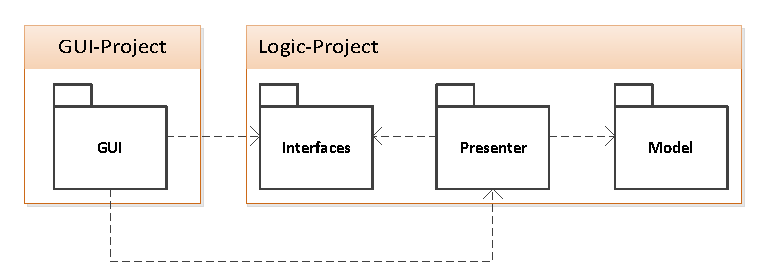
\includegraphics[width=\textwidth]{gfx/mvp.pdf}
\caption{\ac{MVP}-Pattern}
\label{fig:mvp}
\end{center}
\end{figure}

This already show the division into two distinct projects:

\begin{description}
\item[GUI:] Hosts the \ac{GUI} implemented in WinForms. This includes all display-related logic: perform actions based on events, display and hide controls, respond to clicks.
\item[Logic:] Hosts the \textit{business}-logic, the interfaces and the presenters.
\end{description}

As can already be inferred from the short description, most of the application's logic is based in the logic project, which (excluding the view interfaces) encompasses the following classes:

\begin{figure}[H]
\begin{center}
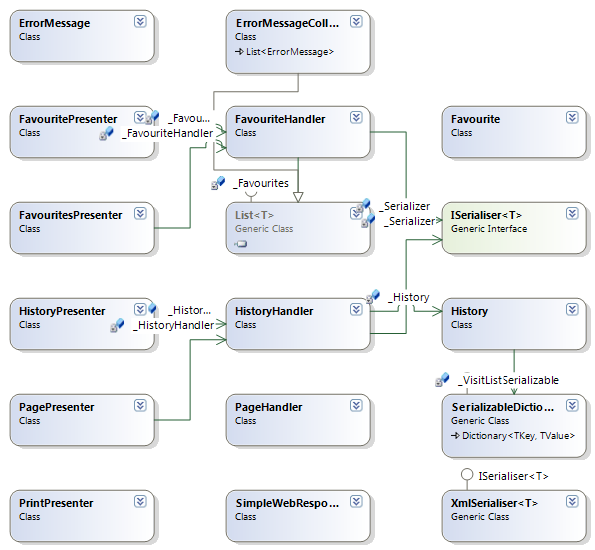
\includegraphics[width=\textwidth]{gfx/class_diagram.png}
\caption{Classes of the logic project.}
\label{fig:mvp}
\end{center}
\end{figure}

The following design decisions were made while implementing the application:

\section{Separate change}
\label{subsec:separate_change}

Special attention should be paid to the classes \texttt{FavouriteHandler} and \texttt{HistoryHandler}.
From a design point-of-view, they provide the presenters that are utilizing them with a facade to the data-classes \texttt{History} and \texttt{Favourite}.

To centralize changes and prevent data loss due to multiple handlers, both objects were implemented via the \texttt{Singleton} pattern, ensuring only one object is present at any given time. This way all presenters will modify the same data.

Moreover the handler classes implement an \texttt{Observer} pattern to notify the relevant presenter about any changes that occur in the data. This way the presenter can make certain that the view is always displaying accurate data. This was necessary as the \texttt{PagePresenter} and the \texttt{HistoryPresenter} both operate on the history-data: the \texttt{PagePresenter} adds every visited page to the history, whereas the \texttt{HistoryPresenter} ensures that the History is correctly displayed in the view.

The same principle applies in the case of the \texttt{FavouritePresenter} and the \texttt{FavouritesPresenter}. The first one adds and edits one single \texttt{Favourite}, whereas the second presenter handles the display of multiple \texttt{Favourite}s and the deletion logic.

\section{Loose coupling}
\label{subsec:loose_coupling}

To provide a loosely coupled application that may be enhanced with little effort at a later time, the communication between distinct logical groups in the application was implemented via interfaces.

The logical groups (that are not denoted separately in the projects) are:

\begin{itemize}
\item View: Realized in a separate project.
\item Logic: Realized in the logic project.
\item Persistence: Realized in the logic project in the classes \texttt{ISerialiser} and the concrete implementations of the interface.
\end{itemize}

As already shown in the \ac{MVP} pattern the presenter $\longleftrightarrow$ view communication is decoupled via interfaces.
Moreover the logic $\longleftrightarrow$ persistence communication is decoupled via the \texttt{ISerialiser} interface as well.

\section{Threading}
\label{subsec:threading}

To fulfil the requirements \texttt{AR01} and \texttt{AR02} multi threading was introduced in the application when a web-page is requested.

Therefore the request will be carried out in an \texttt{asynchronous} thread.

As the view should not be concerned about concrete implementation choices, the decision was made, to introduce multi-threading in the \ac{logic} project. It is implemented in the \texttt{TextPage}-presenter. This way the application will not loose one of its core-functions should the customer decide to exchange the \ac{GUI}.

However, certain changes had to be implemented in the \ac{GUI} to support multi-threading in a WinForms application (see \autoref{sec:implementation_view} for the details): should the \ac{GUI} be exchanged these problems might need to be taken into account again.